\documentclass[tikz,border=8pt]{standalone}
% Shared look for every TikZ diagram. Load with \input{../../tools/tikz-style.tex}
\usepackage[T1]{fontenc}
\usepackage{lmodern}
\renewcommand{\sfdefault}{lmr}  % diagrams use the same serif as the text
\usetikzlibrary{arrows.meta, positioning, shapes.geometric, calc, fit, backgrounds}
\definecolor{cblue}{HTML}{4C78A8}
\definecolor{corange}{HTML}{F58518}
\definecolor{cgreen}{HTML}{54A24B}
\definecolor{cred}{HTML}{E45756}
\definecolor{cpurple}{HTML}{B279A2}
\definecolor{cgrey}{HTML}{6B6B6B}
\tikzset{
  every picture/.style={font=\sffamily, line width=1.2pt},
  box/.style={draw=#1, fill=#1!12, rounded corners=4pt, align=center, inner sep=7pt, minimum height=1.1cm},
  box/.default=cgrey,
  arrow/.style={-{Stealth[length=3mm]}, draw=cgrey, line width=1.4pt},
  title/.style={font=\sffamily\bfseries\Large},
  note/.style={font=\sffamily\small, text=cgrey, align=center},
}
\AtBeginDocument{\hyphenpenalty=10000 \exhyphenpenalty=10000}

\begin{document}
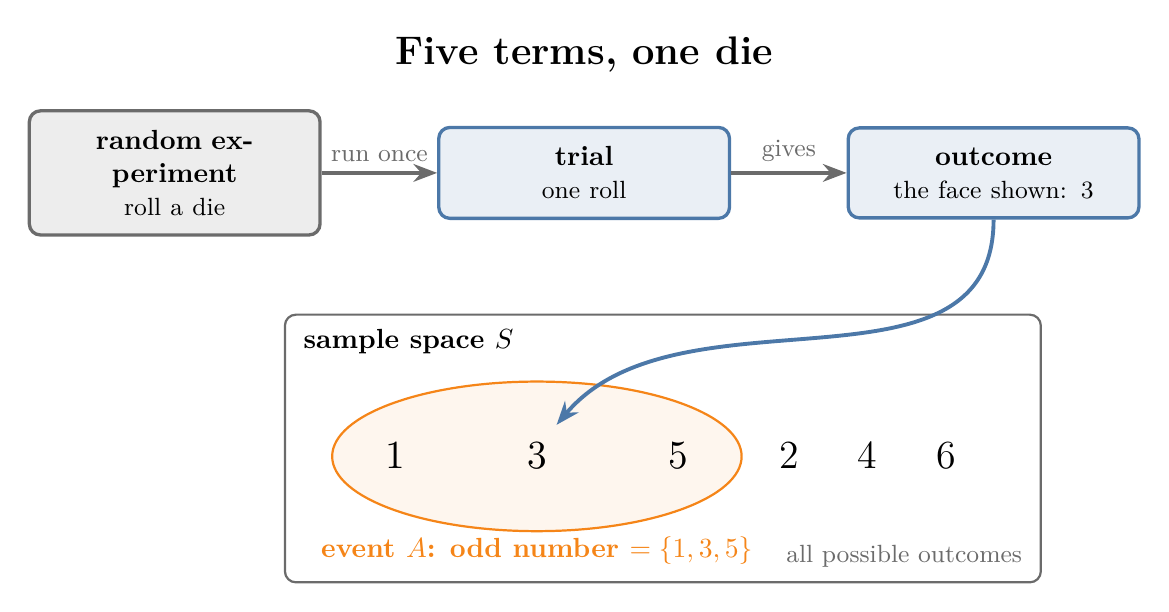
\begin{tikzpicture}[x=1cm, y=1cm]
  \node[title] at (6,5.3) {Five terms, one die};
  \node[box=cgrey, text width=3.2cm] (exp) at (0.8,3.8) {\textbf{random experiment}\\ \small roll a die};
  \node[box=cblue, text width=3.2cm] (tr) at (6,3.8) {\textbf{trial}\\ \small one roll};
  \node[box=cblue, text width=3.2cm] (out) at (11.2,3.8) {\textbf{outcome}\\ \small the face shown: 3};
  \draw[arrow] (exp) -- node[note, above] {run once} (tr);
  \draw[arrow] (tr) -- node[note, above] {gives} (out);
  % sample space
  \draw[thick, rounded corners, draw=cgrey] (2.2,-1.4) rectangle (11.8,2.0);
  \node[font=\sffamily\bfseries, anchor=north west] at (2.3,1.95) {sample space $S$};
  \node[note, anchor=south east] at (11.7,-1.35) {all possible outcomes};
  \foreach \n/\x in {1/3.6,3/5.4,5/7.2,2/8.6,4/9.6,6/10.6} \node[font=\sffamily\Large] (f\n) at (\x,0.2) {\n};
  \draw[thick, corange, fill=corange!12, fill opacity=0.6] (5.4,0.2) ellipse (2.6 and 0.95);
  \foreach \n/\x in {1/3.6,3/5.4,5/7.2} \node[font=\sffamily\Large] at (\x,0.2) {\n};
  \node[text=corange, font=\sffamily\bfseries] at (5.4,-1.0) {event $A$: odd number $=\{1, 3, 5\}$};
  \draw[arrow, draw=cblue] (out.south) to[out=-90, in=50] (5.65,0.6);
\end{tikzpicture}
\end{document}
